\chapter{Implementation}
\label{chap:implementation}

{\small This chapter describes how the methodology of Chapter~\ref{chap:methodology} was realised. Section~\ref{sec:impl_hardware} describes the data basis, from the planned data-collection campaign to the substitute datasets, Section~\ref{sec:impl_software} describes the software implementation, and Section~\ref{sec:impl_optimisation} the measures taken to achieve near-real-time operation on embedded hardware.\par}

\section{Data Collection and Substitute Datasets}
\label{sec:impl_hardware}

\subsection{Planned Data-Collection Campaign}
\label{subsec:impl_go1_plan}

{\small The publicly available datasets considered in this work were recorded with wheeled robots, handheld sensors or in simulation. To evaluate the framework on the type of platform for which it is intended, a dedicated real-world dataset was planned, recorded with a legged robot inside a university building.\par}

{\small An Intel RealSense D455 RGB-D camera~\cite{intel_realsense_d455} was mounted on a Unitree Go1 quadruped robot~\cite{unitree_go1} with a custom 3D-printed base, and the transform between the robot base and the camera was defined manually as the fixed extrinsic $\mathbf{T}_{\mathrm{BC}}$ of Section~\ref{sec:method_preprocessing}. The camera was connected via USB to a Raspberry Pi onboard the robot, which ran the RealSense driver under ROS~1 Melodic, in line with the ROS~1-based software stack of the Go1. A separate onboard computer subscribed to the colour, depth and calibration messages over the internal network of the robot and recorded them at $640 \times 480$ pixels, together with the depth-to-colour extrinsics and the robot odometry, as ROS~1 bags. Depth was recorded in its native sensor geometry rather than aligned to the colour image, which kept the processing load on the Raspberry Pi low, while the recorded extrinsics retained the information required for a later alignment. Since the onboard storage was insufficient for RGB-D recordings, the bags were to be written to an external USB storage device.\par}

{\small The bags were then to be converted into the ROS~2 format and replayed offline through the ROS~2 pipeline~\cite{macenski2022ros2} on the Jetson platform. A live deployment would require either a native ROS~2 interface on the robot or a ROS~1--ROS~2 bridge. The campaign was carried out but ultimately discarded for the reasons described in Section~\ref{subsec:impl_go1_limitations}.\par}

\subsection{Limitations Encountered}
\label{subsec:impl_go1_limitations}

{\small
\begin{table}[htbp]
\centering
\footnotesize
\setlength{\tabcolsep}{4pt}
\caption{Limitations encountered during the Go1 data-collection campaign.}
\label{tab:go1_limitations}
\begin{tabular}{@{}c p{0.17\textwidth}p{0.36\textwidth}p{0.36\textwidth}@{}}
\toprule
\textbf{No.} & \textbf{Limitation} & \textbf{Cause} & \textbf{Consequence} \\
\midrule
1 & \raggedright Onboard compute & \raggedright No power supply or interface for the Jetson AGX Thor on the Go1 & \raggedright Offline processing only \tabularnewline
2 & \raggedright USB bandwidth & \raggedright USB~2.0 only; D455 at 5, 15 or 30\,fps ($640 \times 480$) & \raggedright Frame loss; approx.\ 11.7\,Hz colour and 10.7\,Hz depth at 15\,fps, varying between runs \tabularnewline
3 & \raggedright Vibration & \raggedright Gait vibrations amplified by the 3D-printed mount & \raggedright High depth noise; camera transform not rigid \tabularnewline
4 & \raggedright Reflections & \raggedright Reflective floors and surfaces & \raggedright Critical errors in active stereo depth \tabularnewline
\bottomrule
\end{tabular}
\end{table}
\par}

{\small The limitations summarised in Table~\ref{tab:go1_limitations} fall into three categories. Limitation~1 concerns platform integration; it restricts the campaign to offline evaluation but does not prevent it. Limitation~2 concerns data recording and prevented the complete, temporally consistent streams that the frame preparation of Section~\ref{sec:method_preprocessing} requires. Limitations~3 and~4 concern the quality of the depth measurements.\par}

{\small The depth-quality limitations were decisive, since the framework depends on metric depth at every stage of the per-frame path. Depth is used to back-project segmentation masks into 3D observations (Section~\ref{subsec:method_proposals}), it provides the 3D evidence on which data association is based (Section~\ref{subsec:method_association}), and it is integrated by Hydra into the volumetric reconstruction from which the mesh, the object nodes and the places are derived~\cite{hughes2022hydra}. In addition, back-projection relies on the rigid camera transform of Equation~\eqref{eq:camera_pose}, which the vibrations of limitation~3 invalidate. Noisy depth therefore propagates into the object geometry, the tracking and the map itself. Together with the incomplete recordings, this made the Go1 data unsuitable as the basis of the evaluation.\par}

\subsection{Substitute Datasets}
\label{subsec:impl_datasets}

{\small The substitute datasets were selected according to the input contract of Section~\ref{sec:method_preprocessing}: registered colour and depth images, the camera calibration, odometry and a known base-to-camera extrinsic, recorded in indoor environments as replayable ROS bags.\par}

{\small The office sequences of the OpenLORIS-Scene dataset~\cite{shi2020openloris} serve as the real-world data and are the closest substitute for the planned recordings. They were captured with a RealSense D400-series camera, the sensor family of the D455, and provide depth aligned to the colour image, real wheel odometry and a calibrated base-to-camera transform. Since they were recorded on a wheeled robot with complete sensor streams, they avoid the recording and vibration problems of Section~\ref{subsec:impl_go1_limitations}, so that the method can be evaluated on real sensor data without the results being dominated by these hardware-specific effects.\par}

{\small The simulated office and apartment scenes of the uHumans2 dataset~\cite{rosinol2021kimera}, both with ground-truth odometry and metric depth, complement the real-world data. The office scene was used for development, optimisation and repeatable experiments, while the apartment scene, which contains a human, tests the portability of the framework to a second environment and its handling of a dynamic object. Switching between the datasets requires only configuration (Section~\ref{subsec:impl_portability}). As a consequence of the substitution, effects of legged locomotion, such as gait-induced camera motion and depth noise on reflective floors, are not covered by the evaluation, and the uHumans2 experiments rely on ground-truth odometry (Chapter~\ref{chap:evaluation}).\par}
























% ===========================================================================
% Section 4.2 -- Software Implementation
% Standalone file: include with \input{Section_4_2_Software_Implementation}
% inside the Implementation chapter, after Section 4.1.
% Figures follow claude/DIAGRAM_SPECIFICATIONS.md (five figures).
% ===========================================================================

\section{Software Implementation}
\label{sec:impl_software}

{\small This section describes how the framework of Chapter~\ref{chap:methodology} is realised in software. It follows the components in the order of the data flow, namely the preprocessor, the Phase~1 semantic coordinator with its tracker and labelling lifecycle, Hydra, and the scene graph fuser, and concentrates on their class structure, their concurrency, and the configuration values of the evaluated runs. The design rationale is given in Chapter~\ref{chap:methodology} and is not repeated here.\par}

% ---------------------------------------------------------------------------
\subsection{Package Structure and Deployment}
\label{subsec:impl_deployment}

{\small The framework is implemented as a single ROS~2 package, \texttt{rsg}~\cite{macenski2022ros2}, and runs as a chain of four components, shown together with their classes in Figure~\ref{fig:impl_class_overview}. The preprocessor turns the raw sensor streams into prepared frames and publishes them as the custom message \texttt{RsgFrame}. The Phase~1 semantic coordinator segments and tracks the objects in each frame and passes slot-ID images to Hydra~\cite{hughes2022hydra} on its standard image topics. Hydra builds the scene graph and publishes it as \texttt{hydra\_\allowbreak{}msgs/\allowbreak{}DsgUpdate} to the scene graph fuser, which also receives the label events, heartbeats, and deletion events of the asynchronous semantic path as JSON over \texttt{std\_\allowbreak{}msgs/\allowbreak{}String}. The preprocessor and the coordinator are written in Python; the fuser is written in C++, since it traverses Hydra's complete scene graph through the \texttt{spark\_\allowbreak{}dsg} library. Hydra and the llama.cpp server~\cite{llamacpp} that hosts the VLM run as separate processes. % TODO: confirm the ROS 2 distribution of the final runs on the Jetson AGX Thor.
\par}

\begin{figure}[p]
    \centering
\makebox[\textwidth][c]{%
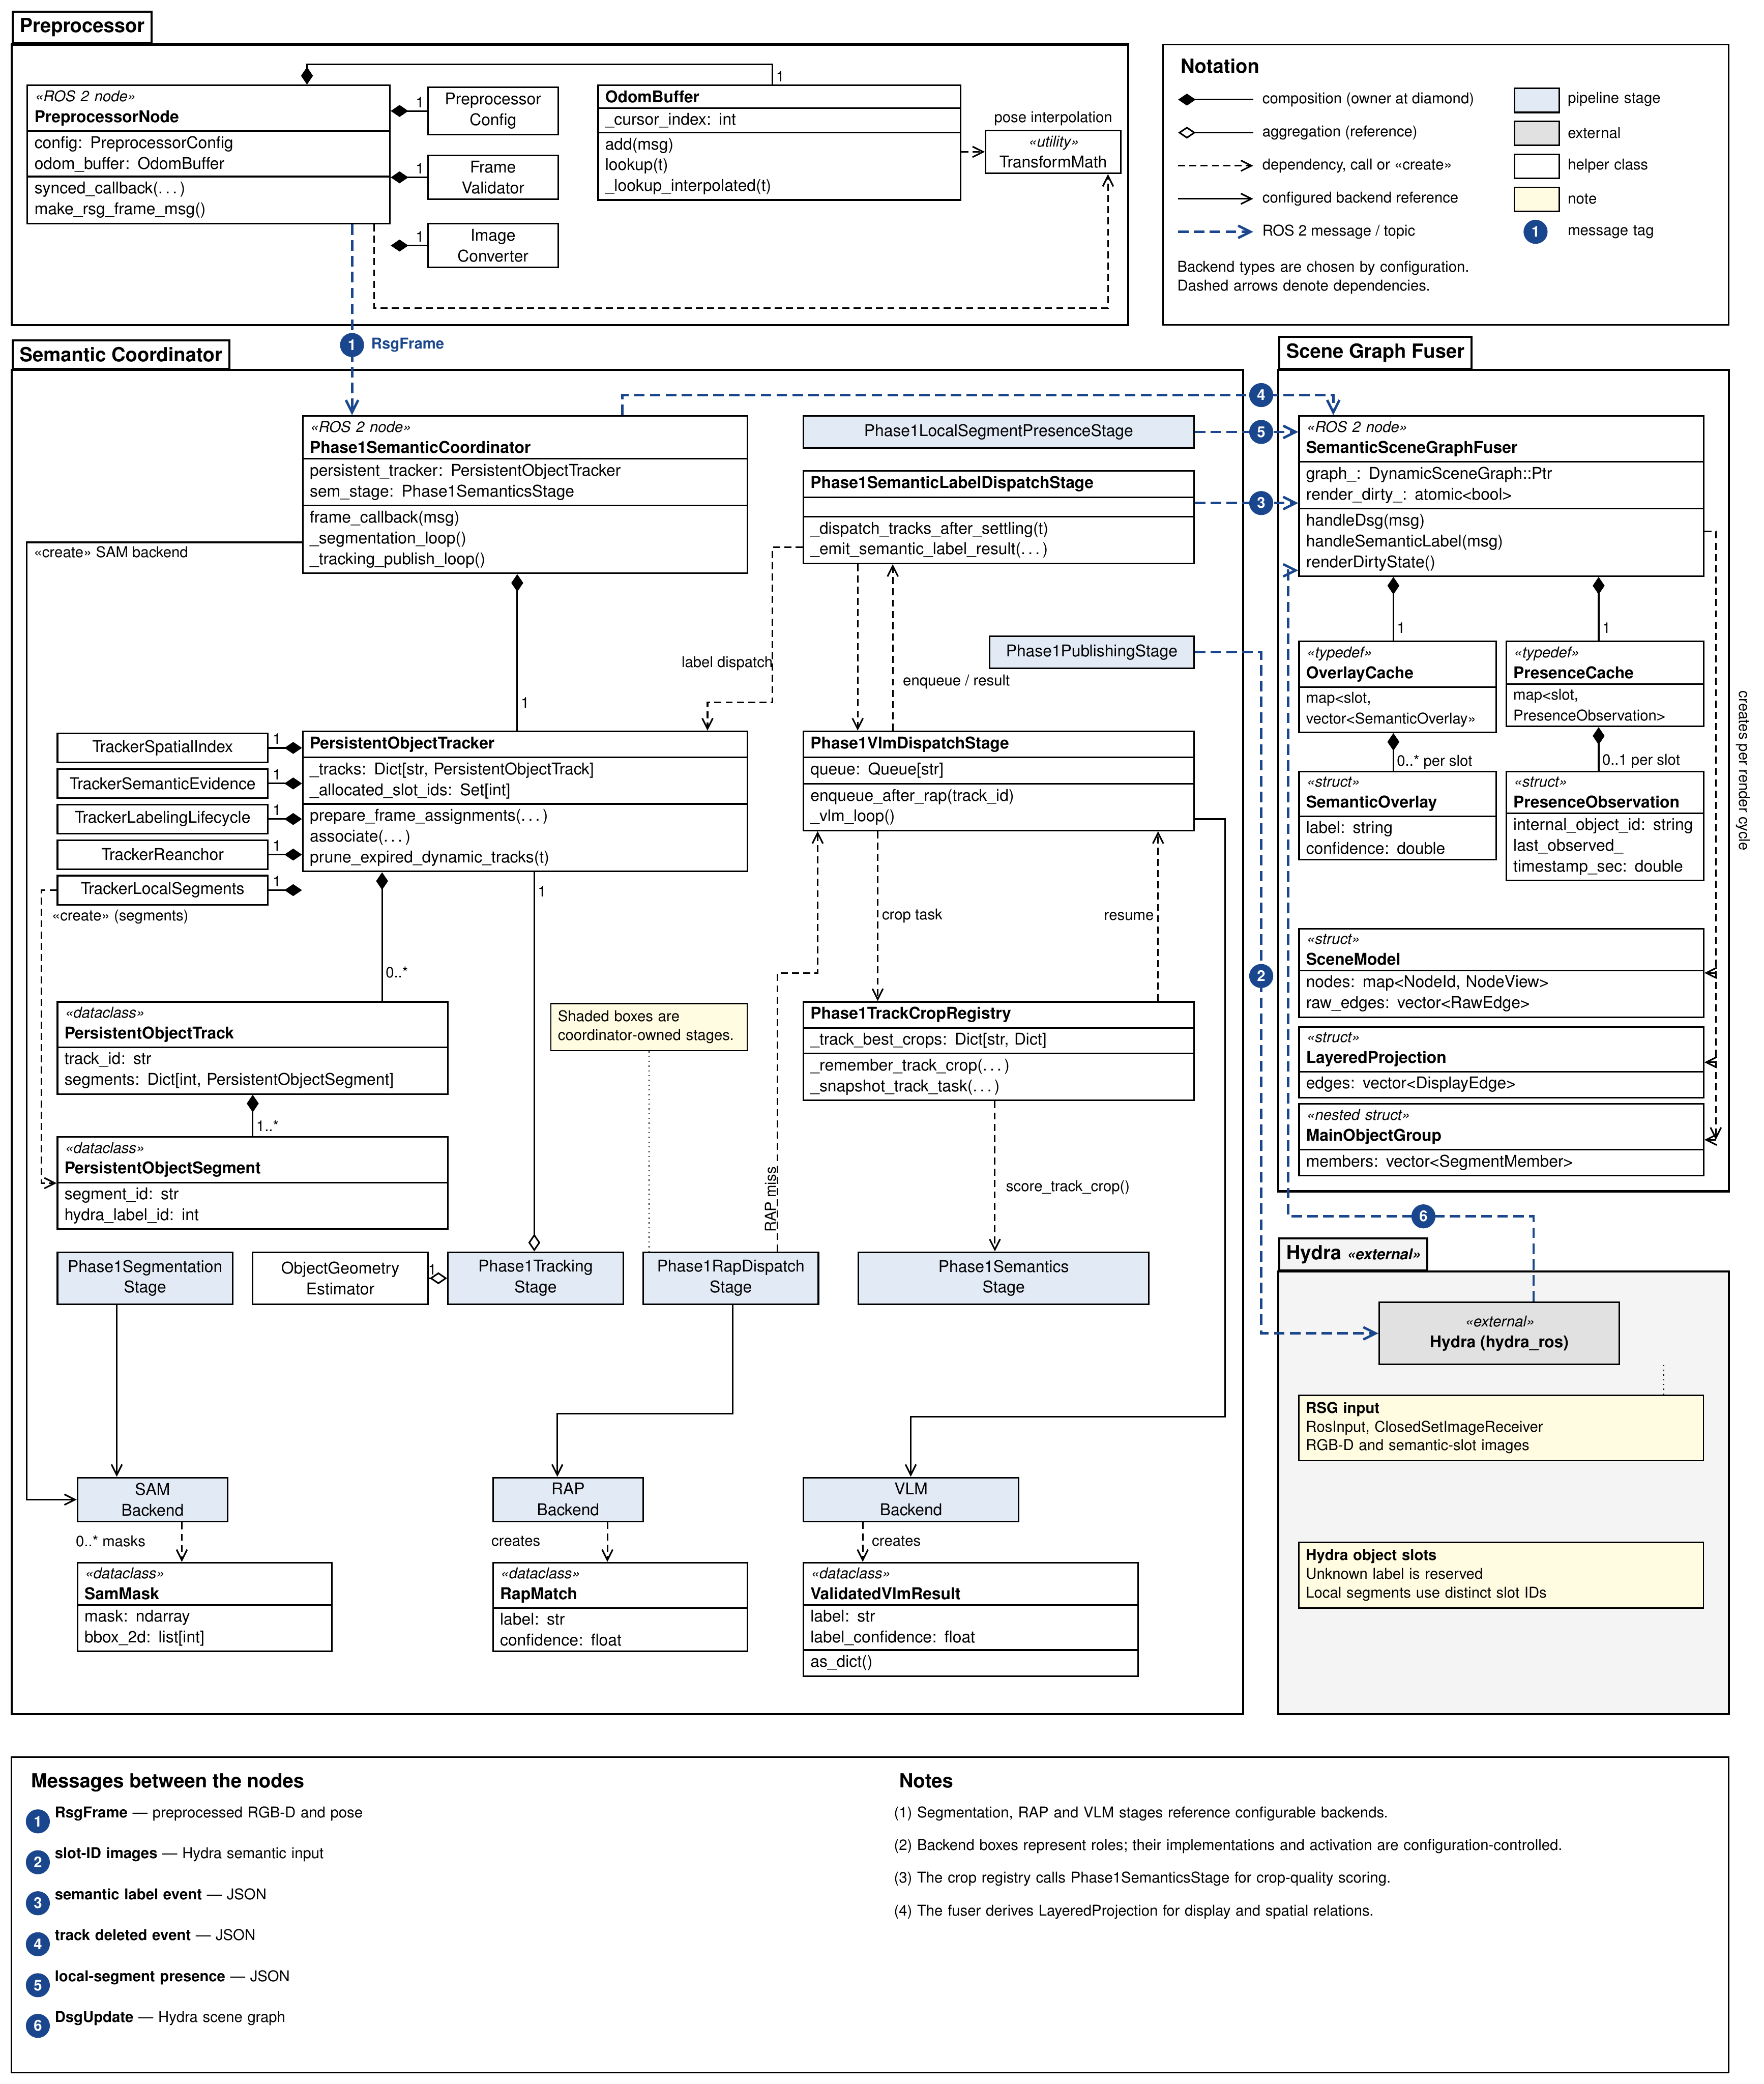
\includegraphics[
            width=\dimexpr\textwidth+3.4cm\relax,
            height=\dimexpr\textheight-1.9cm\relax,
            keepaspectratio
        ]{example_images/impl_class_overview.png}
    }
\caption{Class overview of the implemented framework,
    showing the main ROS~2 nodes, internal processing stages,
    supporting classes, and configurable backends.}
\label{fig:impl_class_overview}
\end{figure}

{\small Within each node, the ROS~2 node class handles only subscriptions, publications, and threads, and delegates the processing to separate classes. In the coordinator, this takes the form of a stage-based architecture: each step of the Phase~1 pipeline is a stage class in its own module, for example \texttt{Phase1\allowbreak{}Segmentation\allowbreak{}Stage}, \texttt{Phase1\allowbreak{}Vlm\allowbreak{}Dispatch\allowbreak{}Stage}, or \texttt{Phase1\allowbreak{}Publishing\allowbreak{}Stage}. The coordinator composes the stages at start-up and keeps only the state they share, namely the tracker and the queues between its threads. Models are reached through backend interfaces selected by factory functions, so that a stage or a model can be exchanged without affecting the rest of the pipeline (Section~\ref{subsec:impl_portability}).\par}

{\small All settings that differ between datasets or models are kept in configuration files rather than in code. A run is defined by a pipeline file, whose \texttt{preprocessing} and \texttt{phase1} sections are read by the preprocessor and the coordinator, a fuser file, and Hydra's input file, dataset file, and slot-only label space. The launch file \texttt{rsg\_\allowbreak{}all.\allowbreak{}launch.\allowbreak{}py} selects these files through launch arguments, with one set each for uHumans2 and OpenLORIS. Within the pipeline file, the VLM is chosen by a profile: \texttt{phase1.\allowbreak{}vlm.\allowbreak{}profiles} defines one entry per model, with its endpoint, model file, server arguments, and memory requirement, and \texttt{active\_\allowbreak{}profile} selects the entry used by both the coordinator and the script that starts the llama.cpp server.\par}

% ---------------------------------------------------------------------------
\subsection{Preprocessor}
\label{subsec:impl_preprocessor}

{\small \texttt{PreprocessorNode} holds a \texttt{Preprocessor\allowbreak{}Config} and delegates temporal association to \texttt{OdomBuffer}, the validity checks to \texttt{FrameValidator}, image handling to \texttt{ImageConverter}, and rigid-body arithmetic to the stateless \texttt{TransformMath} (Figure~\ref{fig:impl_class_overview}). Figure~\ref{fig:impl_seq_preprocessor} shows the processing of one frame. Odometry messages are appended to \texttt{OdomBuffer} as they arrive, and the latest calibration is cached outside the image synchroniser. RGB and depth images are paired by a \texttt{message\_\allowbreak{}filters} approximate-time synchroniser. A synchronised pair is rejected if no calibration is available or if the resolutions of RGB and depth differ, and it is skipped if it would exceed the configured maximum output rate.\par}

\begin{figure}[htbp]
  \centering
  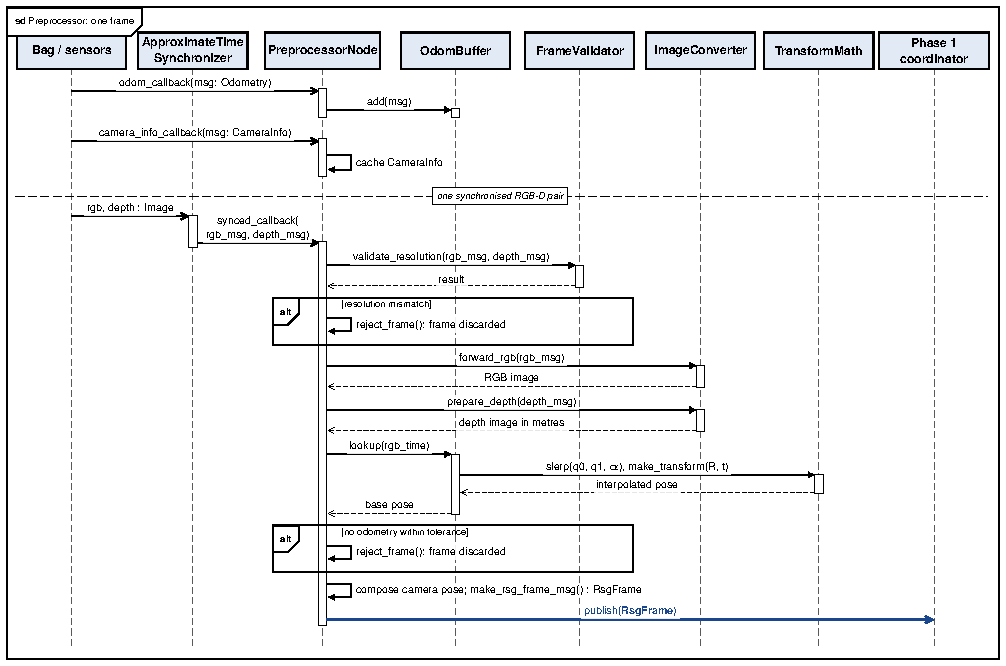
\includegraphics[width=\textwidth]{example_images/impl_seq_preprocessor.pdf}
  \caption{Sequence of one frame through the preprocessor.}
  \label{fig:impl_seq_preprocessor}
\end{figure}

{\small Images that already satisfy the output contract (\texttt{rgb8}, and \texttt{32FC1} in metres) are forwarded by reference; depth recorded in millimetres is converted to metres. Since frames arrive in temporal order, \texttt{OdomBuffer} advances a cursor instead of searching the buffer. It interpolates the base pose linearly in translation and by spherical linear interpolation in rotation, falls back to the nearest sample if no enclosing pair exists, and rejects the frame if no sample lies within the configured time tolerance. The camera pose is obtained by composing the interpolated base pose with the fixed transform $\mathbf{T}_{\mathrm{BC}}$, after which the node assembles and publishes one \texttt{RsgFrame}. For datasets whose bags contain no dynamic transform stream, the node also broadcasts the camera transform. For replay, QoS override files republish \texttt{/\allowbreak{}tf\_\allowbreak{}static} and the latched calibration as \texttt{TRANSIENT\_\allowbreak{}LOCAL}, so that late subscribers such as Hydra still receive them.\par}

% ---------------------------------------------------------------------------
\subsection{Phase~1 Coordinator}
\label{subsec:impl_phase1}
\label{subsec:impl_tracker}
\label{subsec:impl_labelling}

{\small \texttt{Phase1\allowbreak{}Semantic\allowbreak{}Coordinator} loads its configuration, creates the model backends through the factory functions \texttt{make\_\allowbreak{}sam\_\allowbreak{}backend}, \texttt{make\_\allowbreak{}rap\_\allowbreak{}backend}, and \texttt{make\_\allowbreak{}vlm\_\allowbreak{}backend}, and composes one object per pipeline stage (Figure~\ref{fig:impl_class_overview}). Stages and backends exchange data only through the data classes \texttt{SamMask}, \texttt{RapMatch}, and \texttt{ValidatedVlmResult}. The coordinator is organised as a pipeline of threads connected by bounded queues, whose interaction is shown in Figure~\ref{fig:impl_seq_phase1}. Five threads are active: the ROS executor, a segmentation thread, a tracking/publish thread, a RAP worker, and a VLM worker.\par}

{\small The per-frame path is split into two stages that run on separate threads and form a two-stage pipeline: a segmentation stage and a tracking/publish stage. While the segmentation thread processes frame~$n+1$, the tracking/publish thread processes frame~$n$. The split follows the nature of the work: segmentation is GPU-bound and releases the global interpreter lock while it waits for inference, whereas tracking and publication are CPU-bound, so that the two stages overlap in time and the frame rate is limited by the slower stage rather than by the sum of both.\par}

{\small The executor callback wraps each \texttt{RsgFrame} and places it in \texttt{frame\_\allowbreak{}fifo}, from which the segmentation thread takes it, converts the images and calls the segmentation backend through \texttt{Phase1\allowbreak{}Segmentation\allowbreak{}Stage}, which downscales the image, runs the segmenter, and restores the masks to full resolution. The result is passed through \texttt{sam\_\allowbreak{}output\_\allowbreak{}fifo} to the tracking/publish thread. Both queues deliberately hold a single entry and drop the oldest one when full: if the receiving thread is still busy, the waiting frame is replaced by the newer one, so that only the most recent frame is processed. Larger queues would avoid these drops, but every frame they buffer would delay the output passed to Hydra, so that the latency of the map would grow whenever processing falls behind the frame rate and near-real-time operation would be lost. The tracking/publish thread first computes a 3D observation for every mask with \texttt{Object\allowbreak{}Geometry\allowbreak{}Estimator}, which back-projects a subsample of the pixels of the largest connected region within the valid depth range and discards masks with too few valid points. It then assigns all observations of the frame jointly with \texttt{Persistent\allowbreak{}Object\allowbreak{}Tracker} and offers each crop to \texttt{Phase1\allowbreak{}Track\allowbreak{}Crop\allowbreak{}Registry}, which keeps the best crop of each track according to Equation~\ref{eq:crop_score}.\par}

{\small Before the frame is published to Hydra, the same thread performs the bookkeeping of the asynchronous path. \texttt{Phase1\allowbreak{}Local\allowbreak{}Segment\allowbreak{}Presence\allowbreak{}Stage} publishes the heartbeat of the slots observed in the frame, \texttt{Phase1\allowbreak{}Semantic\allowbreak{}Label\allowbreak{}Dispatch\allowbreak{}Stage} schedules tracks whose settling period has elapsed, weak crops whose waiting time has expired are released to the VLM, and confirmed dynamic tracks whose presence confidence has decayed are deleted, which is announced to the fuser as a \texttt{track\_\allowbreak{}deleted} event on the label topic. Finally, \texttt{Phase1\allowbreak{}Publishing\allowbreak{}Stage} renders the masks into \texttt{16UC1} semantic and instance images of slot identifiers in decreasing order of mask area, sets depth and label to zero outside the valid depth range, and publishes RGB, depth, label images, and calibration to Hydra with the original timestamp. The tracker lock and a re-entrant lock on the crop registry guard the state shared with the RAP and VLM workers. Python threads suffice, since TensorRT inference and blocking HTTP requests release the global interpreter lock.\par}

% Both parts on one float page; requires \usepackage{graphicx} and \usepackage{subcaption}.
\begin{figure}[p]
  \centering
  \begin{subfigure}{\textwidth}
    \centering
    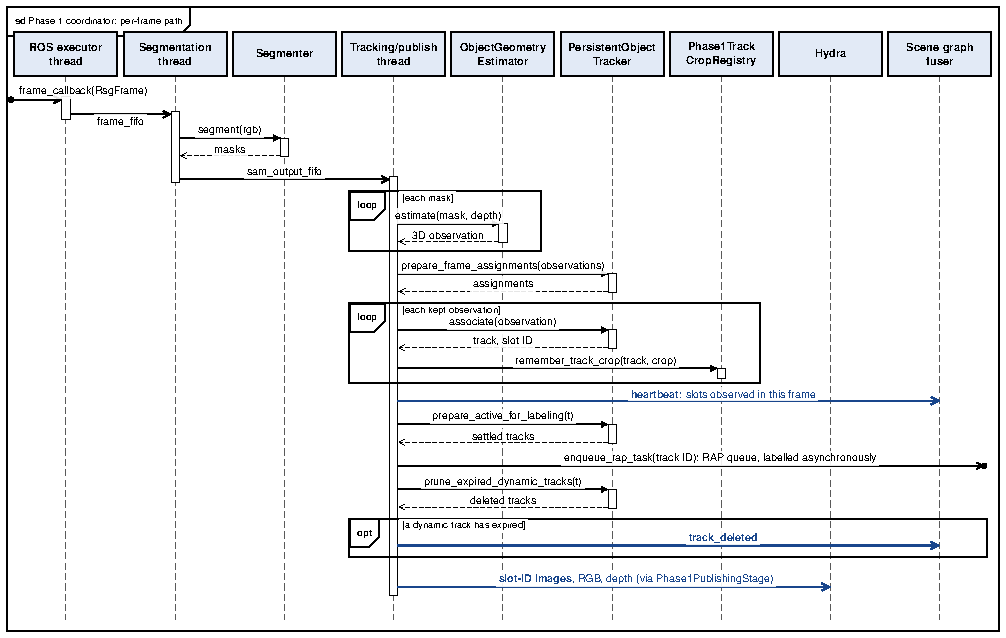
\includegraphics[width=\textwidth,height=0.41\textheight,keepaspectratio]{example_images/impl_seq_phase1_frame.pdf}
    \caption{Synchronous per-frame path.}
    \label{fig:impl_seq_phase1_frame}
  \end{subfigure}

  \vspace{0.6\baselineskip}

  \begin{subfigure}{\textwidth}
    \centering
    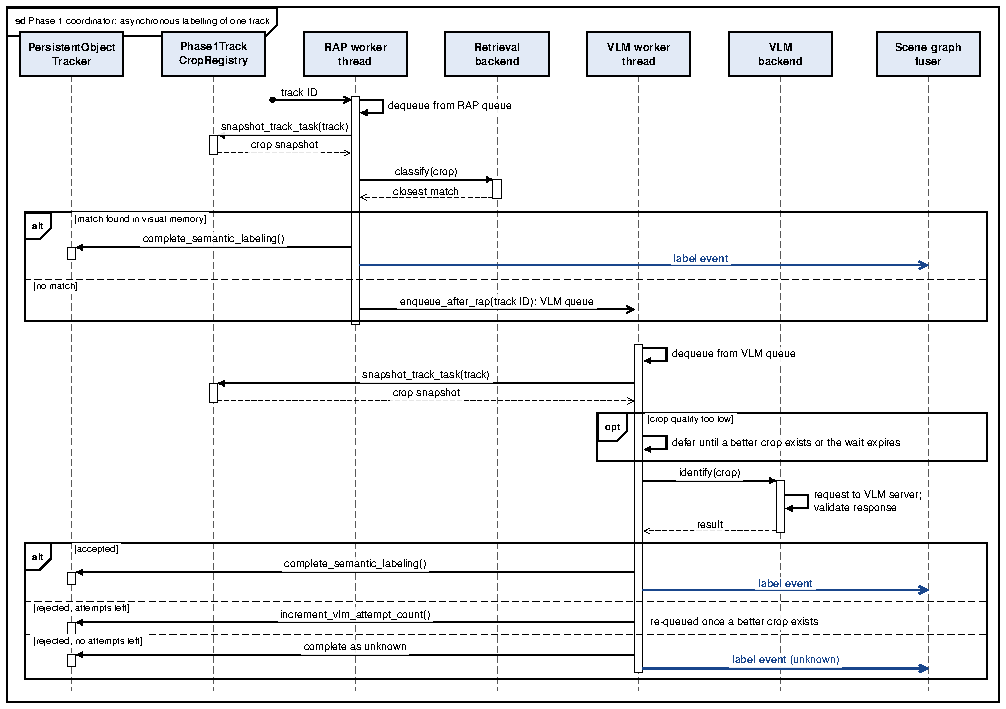
\includegraphics[width=\textwidth,height=0.455\textheight,keepaspectratio]{example_images/impl_seq_phase1_label.pdf}
    \caption{Asynchronous labelling of one track by the RAP and VLM workers.}
    \label{fig:impl_seq_phase1_label}
  \end{subfigure}
  \caption{Sequence of the Phase~1 coordinator.}
  \label{fig:impl_seq_phase1}
\end{figure}

{\small The track state of Section~\ref{subsec:method_track_state} is held in \texttt{Persistent\allowbreak{}Object\allowbreak{}Track} objects, each of which owns one or more \texttt{Persistent\allowbreak{}Object\allowbreak{}Segment} objects whose field \texttt{hydra\_\allowbreak{}label\_\allowbreak{}id} stores the slot ID. The joint assignment of Equation~\ref{eq:assignment} is implemented in \texttt{prepare\_\allowbreak{}frame\_\allowbreak{}assignments}, which selects the track for each observation with \texttt{\_greedy\_maximize}. For persistence across sessions (Section~\ref{subsec:method_sessions}), the module \texttt{tracker\_\allowbreak{}state\_\allowbreak{}store} writes the tracker state atomically to a versioned JSON file; on restoration, the timestamps are shifted into the past, so that restored tracks are matched in revisit mode.\par}

{\small The labelling scheme of Section~\ref{sec:method_overview} is realised by \texttt{Phase1\allowbreak{}Semantic\allowbreak{}Label\allowbreak{}Dispatch\allowbreak{}Stage} together with \texttt{Phase1\allowbreak{}Rap\allowbreak{}Dispatch\allowbreak{}Stage} and \texttt{Phase1\allowbreak{}Vlm\allowbreak{}Dispatch\allowbreak{}Stage} (Figure~\ref{fig:impl_seq_phase1_label}), and its progress is recorded in the \texttt{labeling\_\allowbreak{}status} of each track. When a worker queue is full, identifiers are deferred rather than dropped, so that no track loses its labelling request. Before a VLM request, the crop additionally passes a quality gate based on size, border contact, and crop score; a track that fails it waits in \texttt{vlm\_\allowbreak{}waiting\_\allowbreak{}for\_\allowbreak{}better\_\allowbreak{}crop} until a better crop is registered or a maximum waiting time has passed. Validation is implemented in \texttt{validate\_\allowbreak{}vlm\_\allowbreak{}response}, and an accepted result is published as one label event per slot of the track.\par}


% ---------------------------------------------------------------------------
\subsection{Hydra Integration and Session Persistence}
\label{subsec:impl_hydra}

{\small Hydra is configured with the frozen label space \texttt{rsg\_\allowbreak{}slot\_\allowbreak{}only\_\allowbreak{}frozen\_\allowbreak{}label\_\allowbreak{}space.\allowbreak{}yaml}, which contains the background label and the slots 1 to 10\,000, all declared as object labels, with a dataset configuration that holds the map parameters, and with an input configuration that connects Hydra's image receiver to the Phase~1 topics. Figure~\ref{fig:impl_seq_hydra} shows the resulting sequence. Since every slot is an object label, Hydra clusters one object per slot, so that object identity is decided by Phase~1 rather than by Hydra's class labels. The modifications of Section~\ref{subsec:method_architecture} are implemented as follows. Both the receiver queue and the input queue of the active window are bounded to five entries and filled without blocking, so that frames are dropped when reconstruction falls behind instead of accumulating a backlog. Since segmentation often detects an object only after it has been seen in several frames, its voxels first receive evidence for the background label. Hydra's maximum-likelihood semantic integrator accumulates this evidence without decay, so that such a head start could prevent the object's slot label from ever prevailing and the object would never form a node. The integrator was therefore modified to ignore the background label: a voxel that has only been observed as background remains undetermined, while competition between object labels is unaffected.
\par}

{\small For resumption, the saved scene graph and mesh are loaded into the back-end before integration, restored nodes are archived so that re-observations are merged into them, node identifiers continue after the restored ones, and back-end object merging is enabled. At shutdown, the back-end writes the scene graph, the mesh, and the deformation graph, and the active window writes its volumetric map. Session state is kept in three stores under \texttt{memory/} (tracker JSON, Hydra back-end files, Chroma directory), which are controlled by one switch and cleared by \texttt{clear\_\allowbreak{}memory.\allowbreak{}py}; in the evaluated configuration, this switch is disabled, so that every run starts from an empty map. For loop closure, the coordinator latches the \texttt{map}-to-\texttt{odom} transform from \texttt{/\allowbreak{}tf}, ignores changes below configured translation and rotation thresholds, and otherwise calls \texttt{reanchor\_\allowbreak{}all} and \texttt{merge\_\allowbreak{}reanchor\_\allowbreak{}duplicates}; with ground-truth odometry, this hook remains inert.\par}

\begin{figure}[htbp]
  \centering
  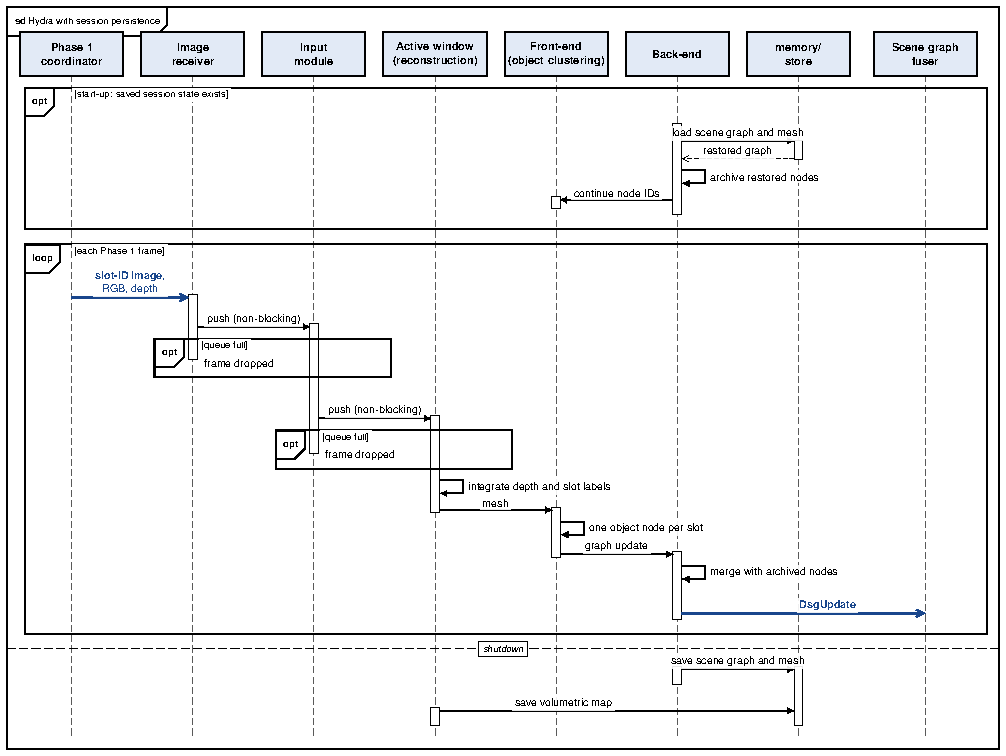
\includegraphics[width=\textwidth]{example_images/impl_seq_hydra.pdf}
  \caption{Sequence of the modified Hydra pipeline with session persistence.}
  \label{fig:impl_seq_hydra}
\end{figure}

% ---------------------------------------------------------------------------
\subsection{Scene Graph Fuser}
\label{subsec:impl_fuser}

{\small The scene graph fuser, implemented as the class \texttt{Semantic\allowbreak{}Scene\allowbreak{}Graph\allowbreak{}Fuser}, joins Hydra's geometry and the semantic events of Phase~1 by slot ID. Since the two streams arrive independently, for instance a label before its object node exists, the fuser does not combine them on arrival but stores them in shared state: a local copy of Hydra's scene graph, the overlay and presence caches of each slot, the set of deleted slots, and the flag \texttt{render\_\allowbreak{}dirty}, all of which are protected against simultaneous access. Three concurrent callback groups interact only through this state (Figure~\ref{fig:impl_seq_fuser}). The graph callback group applies Hydra's \texttt{DsgUpdate} messages to the local graph, either replacing it or applying an incremental update with its deletions. The semantic callback group stores label events and \texttt{track\_\allowbreak{}deleted} events in the overlay cache and the set of deleted slots, and heartbeats in the presence cache. Both groups merely store the data and set the flag, so that ingestion is never blocked by rendering.\par}
\begin{figure}[htbp]
  \centering
  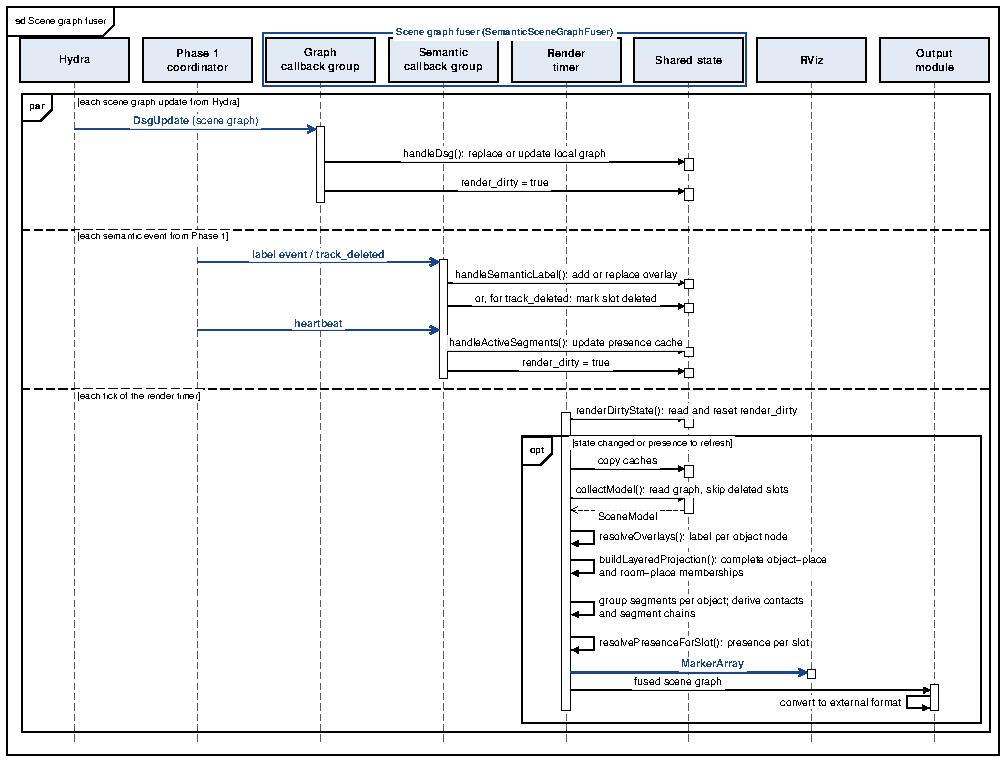
\includegraphics[width=\textwidth]{example_images/impl_seq_fuser.pdf}
  \caption{Sequence of the scene graph fuser.}
  \label{fig:impl_seq_fuser}
\end{figure}
{\small The third group, a periodic timer, renders only if the flag is set or presence confidences have to be refreshed, so that several messages within one period cause a single render. It first copies the caches, so that it works on a consistent snapshot while new messages continue to arrive. From this snapshot and the local graph, it derives the scene model without the deleted slots and assigns a label to each object node, so that a label that arrived early is applied as soon as its node exists. It then completes missing object--place memberships, validated against the mesh, and room--place memberships, groups the segments of each physical object to derive contacts between objects and the chains between their segments, and resolves the presence of each slot according to Equation~\ref{eq:presence_decay}. The fused scene graph is published as an RViz marker array and passed to an output module, which converts it into a format for external consumers such as a downstream risk assessment.\par}

% ---------------------------------------------------------------------------
\subsection{Portability and Extensibility}
\label{subsec:impl_portability}

{\small The framework separates the models and the dataset from the code, so that each of them can be exchanged through the configuration files described in Section~\ref{subsec:impl_deployment}. The pipeline accesses every model only through a small interface, \texttt{VlmBackend}, \texttt{SamBackend}, or \texttt{RapBackend} (Figure~\ref{fig:impl_class_overview}), and a factory function creates the implementation named in the pipeline configuration file at start-up. The following paragraphs describe the steps required to use a new VLM, a new segmentation model, and a new dataset.\par}

{\small \textbf{New VLM.} A VLM that is served through an OpenAI-compatible chat-completions endpoint, as provided by llama.cpp~\cite{llamacpp}, requires no change to the code. A new entry is added under \texttt{phase1.\allowbreak{}vlm.\allowbreak{}profiles} in the pipeline configuration file, specifying the endpoint, the model name, the model file and its vision projector, the server arguments, and the minimum system memory. Setting \texttt{phase1.\allowbreak{}vlm.\allowbreak{}active\_\allowbreak{}profile} to this entry selects the model: at start-up, the launcher \texttt{rsg\_\allowbreak{}vlm\_\allowbreak{}server} checks the available memory and starts the server with the model, and the coordinator sends its requests to the same endpoint. The prompt and the validation thresholds are defined independently of the profiles and therefore remain unchanged; the new model only has to return the same structured output, and its labelling accuracy should be re-validated with the existing prompt. Only a VLM with a different interface requires a new implementation of \texttt{VlmBackend} and an entry in \texttt{make\_\allowbreak{}vlm\_\allowbreak{}backend}.\par}

{\small \textbf{New segmentation model.} The segmentation model is selected by \texttt{phase1.\allowbreak{}sam.\allowbreak{}backend}, and the files of each backend are specified in its own configuration block. A model that is compatible with an existing backend, such as another SAM checkpoint for \texttt{RealSamBackend} or other TensorRT engines for \texttt{NanoSamBackend}, is therefore used by changing these file paths. A model with a different interface requires a new class that implements \texttt{segment(rgb)} and returns the masks as \texttt{SamMask} objects, an entry in \texttt{make\_\allowbreak{}sam\_\allowbreak{}backend} under a new backend name, and a configuration block for its files. Since all later stages consume only \texttt{SamMask} objects, no other part of the pipeline is affected; \texttt{NanoSamBackend} was added alongside \texttt{RealSamBackend} in exactly this way.\par}

{\small \textbf{New dataset.} A new dataset or robot requires only a new set of configuration files and no change to the code. The pipeline configuration file specifies the input topics, the coordinate frames, the fixed transform between the robot base and the camera, and the depth scale of the sensor; the fuser configuration file specifies the parameters of the fused graph; Hydra's input configuration connects its image receiver to the Phase~1 topics and sets the sensor range; and Hydra's dataset configuration contains the map parameters, which have to be tuned to the new sensor. If the data are replayed from bags, a QoS override file republishes static transforms and calibration so that late subscribers still receive them. The new files are passed to \texttt{rsg\_\allowbreak{}all.\allowbreak{}launch.\allowbreak{}py} through the launch arguments \texttt{pipeline\_\allowbreak{}config}, \texttt{fuser\_\allowbreak{}config}, \texttt{input\_\allowbreak{}config}, and \texttt{dataset}. OpenLORIS was added to the framework in this way, without any change to the code used for uHumans2 (Section~\ref{subsec:impl_datasets}).\par}